\documentclass[twocolumn, 11pt]{article}%
\usepackage{amsmath, amssymb, esint, gensymb, hyperref, mathtools}
\usepackage{graphicx, cuted, geometry, float, scalerel, xcolor, xfrac}

\newcommand\sbullet[1][.5]{\mathbin{\ThisStyle{\vcenter{\hbox{%
  \scalebox{#1}{$\SavedStyle\bullet$}}}}}%
}

\geometry{
    a4paper,
    total={170mm,260mm},
}

\begin{document}

\begin{strip}
  \vspace*{\dimexpr-\stripsep}
  \begin{center}
      \Large\textbf{FISIKA 2}\\
      \large{Pertemuan 2 - Minggu 6 (302651)}\\
      \large{\today}
   \end{center}
\end{strip}

\section{Rangkaian Listrik Searah}
\subsection{Hukum Kirchhoff 1}%
    Hukum Kirchhoff 1 menyatakan bahwa jumlah kuat arus yang menuju titik percabangan sama dengan jumlah kuat arus yang meninggalkan titik percabangan.
    \begin{center}
    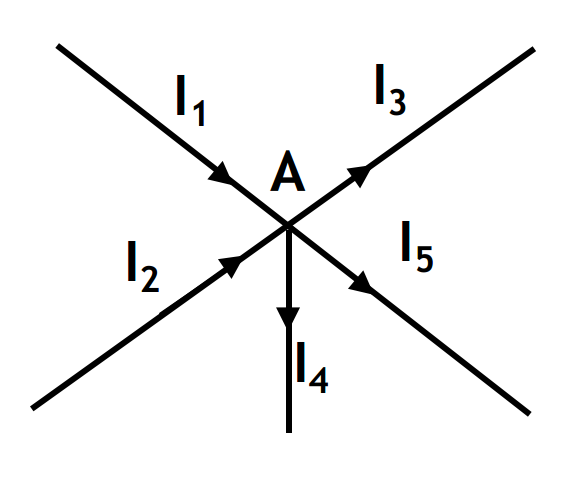
\includegraphics[width=100px]{1.png}
    \end{center}
    \begin{align*}
        \Sigma\ I_{masuk} &= \Sigma\ I_{keluar}\\
        I_1 + I_2 &= I_3 + I_4 + I_5
    \end{align*}
\subsection{Hukum Kirchhoff 2}%
    Hukum Kirchhoff 2 menyatakan bahwa pada loop atau rangkaian tertutup, jumlah potensialnya sama dengan nol.
    \[ \Sigma V=0 \]
    \[\Sigma \epsilon + \Sigma IR=0 \]
    \subsubsection{Satu Loop}%
    \begin{center}
        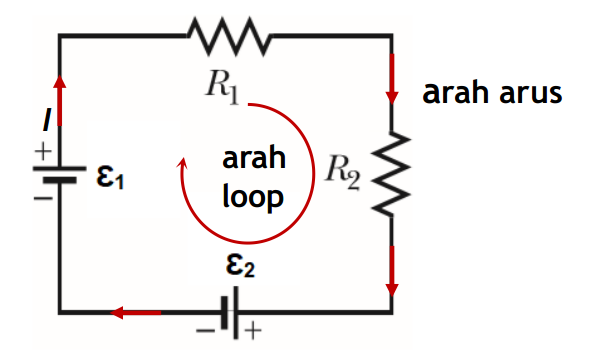
\includegraphics[width=150px]{2.png}
    \end{center}
    \begin{align*}
        \Sigma\epsilon+\Sigma IR&=0\\
        (\epsilon_2-\epsilon_1)+(IR_1+IR_2)&=0\\
        I&=\frac{\epsilon_1-\epsilon_2}{R_1 + R_2}
    \end{align*}

    Masalahnya sekarang adalah tanda, kapan tanda dari sumber GGL itu positif dan kapan tanda resistor itu negatif.\\

    Resistor akan bertanda positif bila \textbf{ARUS DAN LOOP ITU SEARAH}, dan akan bertanda negatif bila \textbf{ARUS DAN LOOP ITU BERLAWANAN}.

    Arah loop itu boleh ditentukan sendiri, yang penting hasil akhirnya positif dengan mengatur arah arus. Bila hasil negatif, arah arus bisa dibalik sehingga hasil akhir perhitungan adalah positif.

    Pada mulanya, buat dulu arah arus sama dengan arah loop (buat aja searah jarum jam dulu). Lalu bila hasilnya negatif, arah arusnya bisa dibalik.\\

    Pada baterai, bila \textbf{PANAH ARAH LOOP MASUK MELALUI KUTUB NEGATIF BATERAI}, maka baterai bernilai negatif. Sebaliknya bila, \textbf{PANAH ARAH LOOP MASUK MELALUI KUTUB POSITIF BATERAI}, maka baterai bernilai positif.

    Menggunakan aturan tanda diatas, bisa pula mencari tegangan jepit antara dua titik dengan rumus umum

    \[V_{AB} = IR_1 + \epsilon_1 \]
    Maksudnya adalah pada potongan antara titik A dan B, arah loop disini melewati Resistor 1 dan Baterai 1. Bila melewati baterai dan resistor lain, $R_1$ atau $\epsilon_1$ bisa diganti dengan $R_2$ atau $\epsilon_2$ atau angka-angka yang lainnya.

    \subsubsection{Dua Loop (Loop Ganda)}%
    Sama dengan rangkaian satu loop, penentuan arah loop pada rangkaian dua loop tetap bisa ditentukan sendiri, asalkan konsisten dan tidak berubah-ubah. 
    \begin{center}
        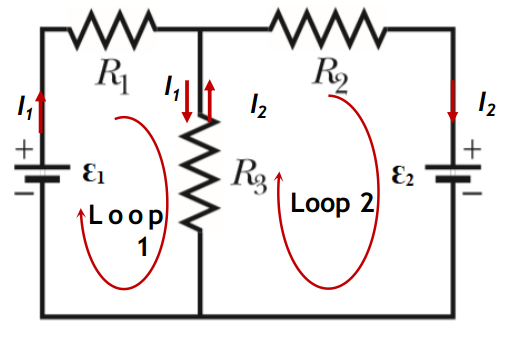
\includegraphics[width=150px]{3.png}
    \end{center}
    
    \textbf{LOOP 1}\\
    \[ -\epsilon_1 + I_1R_1 + (I_1-I_2)R_3=0\]
    \paragraph{}\textbf{LOOP 2}\\
    \[ -\epsilon_2 + I_2R_2 + (I_2-I_1)R_3=0\]

    Untuk aturan loop, aturan arah arus dan aturan tanda pada resistor dan tanda arus sama dengan Rangkaian Satu Loop. Meskipun dengan penentuan arah arus dan arah loop yang berbeda-beda, namun hasil akhirnya pasti sama. Jadi jangan khawatir.

    Pada arus dua loop, akan terbentuk 2 persamaan arus dari masing-masing loop, sehingga bisa dilakukan metode \textbf{eliminasi dan substitusi}.
    
    Untuk menentukan kuat arus pada loop 1 dan loop 2. Untuk mencari arus di setiap percabangannya, bisa digunakan Hukum Kirchhoff 1.

    \subsubsection{Tiga Loop}%
    Secara teori, pada arus tiga loop, hampir sama dengan arus dua loop, namun akan didapatkan TIGA PERSAMAAN arus listrik pada setiap loopnya, sehingga bisa dieliminasi dan disubstitusi.
    
\end{document}
